\documentclass[12pt, a4paper]{article}
\usepackage{triada}
\usepackage{subfigure}
\usepackage{float}
%\usepackage{enumerate}

\graphicspath{{eps/}{png/}}
\begin{document}

\section*{Задание 7}
\subsection*{Постановка}
	Методом случайного поиска найти минимальное значение функции 
	\[ f(x)= x^3\sin\left( \frac 1{x} \right) + 10xy^4\cos\left( \frac 1 {y} \right) \]
	при $x\neq 0,\ y\neq 0$. Функция в нулевых $x$ или $y$ доопределяется по непрерывности.
	Множество поиска --- круг единичного радиуса с центром в нуле. Оценить точность.
\subsection*{Поиск в круге}
Метод случайного поиска заключается в следующем: генерируется достаточно большое количество реализаций случайной величины, равномерно распределенной внутри множества поиска, и ищутся значения функции в полученных точках, среди них находится минимум.

Для генерации случайной величины, равномерно распределенной в круге, будем рассматривать случайную пару точек $(x,y)$, равномерно распределенных в квадрате $[-1,1]\times [-1,1]$. Если пара не попала в круг, т.е. $x^2+y^2>1$, то реализация отбрасывается. Вероятность отбросить пару точек равна отношению площадей круга и квадрата $\frac{\pi}{4}$. Таким образом, для генерации $N$ случайных пар, равномерно распределенных в круге, требуется в среднем сгенерировать $\frac{4N}{\pi}$ равномерных случайных пар из квадрата. 

Оценим теперь точность: пусть $\left(x_*,y_*\right)$ --- точка из выборки, в которой было найдено минимальное значение, $(x_{\min},y_{\min})$ --- точка, в которой достигается минимум. Тогда
\begin{gather*} \left| f(x_{\min} , y_{\min}) - f(x_*,y_*) \right| 
	\leqslant \left| 
	f\left(x_{\min},y_{\min}\right) - f\left(x_{\min},y_*\right)\right| + \left| f\left(x_{\min},y_*\right) - f\left(x_*,y_*\right)  \right| 
	\leqslant \\ \leqslant
	\max\limits_{x,y} \left|f'_{y}\right|\left| y_{\min}-y_*\right| + \max \left|f'_x\right|\left| x_{\min}-x_* \right|, \\
	\max\limits_{x,y} \left|f'_x\right| = \max \left| 3x^2\sin\frac1{x} - x\cos\frac1{x}+10y\cos\frac1y \right|  \leqslant 10 + \sqrt{10}, \\
	\max\limits_{x,y}\left|f'_y\right| = \max \left| 40xy^3\cos\frac1y -10xy^2\sin\frac1y \right| \leqslant 10\sqrt{17}. 
\end{gather*}
Теперь найдем количество элементов, требующееся для достижения некоторой заданной точности $\varepsilon$ с вероятностью $p$. То есть найдем такую величину $\delta$, что вероятность попасть в $\delta$-квадратную окрестность $(x_{\min},y_{\min})$ не меньше $p$.
Итак, вероятность попасть в $\delta$-квадрат вокруг $(x_{\min},y_{\min})$ равна $\frac{\delta^2}{\pi}$. Тогда вероятность не попасть в этот квадрат за $n$ реализаций случайной точки равна $\left(1-\frac{\delta^2}{\pi}\right)^n$. Найдем теперь значение $\delta$, отвечающее точности приближения функции $\varepsilon$.
\[\left| f(x_{\min} , y_{\min}) - f(x_*,y_*) \right| \leqslant \delta\left( 10 + \sqrt{10} + 10\sqrt{17}\right) \approx 55\delta,  \]
поэтому положим $\delta = \frac \varepsilon{55}$, тогда ошибка будет не более $\varepsilon$.

Итоговая формула такова: \[ \left(1-\frac{\varepsilon^2}{55^2\pi}\right)^n \approx \left( 1-0.000105\varepsilon^2 \right) ^n \geqslant 1-p \Rightarrow  n \geqslant \frac{\ln(1-p)}{\ln\left( 1-0.000105\varepsilon^2 \right) }.\] 

Будем в зависимости от $\varepsilon$ и $p$ выбирать количество эффективных(то есть попавших в круг) реализаций и находить минимум методом случайного поиска. Таким образом $n=n_{\text{eff} }\frac{4}{\pi}$.

\begin{tabular}{|l|l|l|l|l|l|l|}
\hline
$\varepsilon$ & $p$ & $n_{\text{eff} }$ & $f_{\min}$ &$x$& $y$ & $x^2+y^2$\\
\hline
$0.5$ & $0.9$ & $87528$ & $-1.2767$ & $-0.3804$ & $-0.9243$& $0.999$ \\
$0.2$ & $0.9$ & $547054$ & $-1.2767$ & $-0.3568$ & $0.9342$ & $0.999$\\
$0.1$ & $0.9$ & $2188219$ & $-1.2880$ & $-0.3574$ & $-0.9339$ & $0.999$\\
$0.05$ & $0.9$ & $8752878$ & $-1.2883$ & $-0.3605$ & $0.9327$ & $0.999$\\
$0.05$ & $0.95$ & $11387757$ & $-1.2882$ & $-0.3587$ & $0.9334$ & $0.999$\\
\hline
\end{tabular}

Функция чётна по $y$, что объясняет тот факт, что минимум находится в одинаковых по модулю, но разных по знаку точках $y$.

Таким образом, с вероятностью $0.95$ число $-1.2882$ отличается от минимального значения $f$ не более чем на $0.05$.

\subsection*{Поиск на окружности}
Полученные выше результаты показывают, что минимум достигается на границе круга. Поэтому можно воспользоваться случайным поиском по окружности для достижения большей точности. Для этого будем достаточно большое число раз генерировать равномерно распределенные на $\left[ 0, 2\pi \right]$ величины $\varphi_i$. Тогда $(x,y) = \left(\cos(\varphi_i),\sin\left(\varphi_i\right)\right)$ будет равномерно распределено на границе круга, в котором предполагался поиск. 

Найдем, как и раньше, зависимость числа случайных величин от вероятности и искомой погрешности. Вероятность не попасть в $\delta$-окрестность некоторой точки равна $1-\frac{2\delta}{\pi}$. Вновь оценивая сверху $\delta$ числом $\frac{\varepsilon}{55}$, получим 
 \[ \left(1-\frac{\varepsilon}{55\pi}\right)^n \approx \left( 1-0.0057\varepsilon^2 \right) ^n \geqslant 1-p \Rightarrow  n \geqslant \frac{\ln(1-p)}{\ln\left( 1-0.0057\varepsilon \right) }.\] 
 
 Нетрудно заметить, при стремлении $\varepsilon$ к нулю при одинаковых $p$ новая оценка на количество случайных величин будет асимптотически медленнее сходиться к бесконечности, что равносильно тому, что новая оценка на $\varepsilon$ при стремлении $n$ к бесконечности будет сходиться к нулю асимптотически быстрее, чем старая. Кроме того, теперь вся выборка точек будет эффективной.

Новая таблица значений приведена ниже.

\begin{tabular}{|l|l|l|l|l|l|l|}
\hline
$\varepsilon$ & $p$ & $n$ & $f_{\min}$ &$x$& $y$ \\
\hline
$0.05$ & $0.9$ & $7956$ & $-1.288489074801$ & $-0.357459414926$ & $0.933928673229$ \\
$0.01$ & $0.95$ & $51761$ & $-1.288489214663$ & $-0.357383456539$ & $-0.933957742615$ \\
$0.001$ & $0.99$ & $795714$ & $-1.288489227599$ & $-0.357351875618$ & $0.933969826596$ \\
$0.0001$ & $0.999$ & $11935741$ & $-1.288489227601$ & $-0.357352110277$ & $0.933969736811$ \\
\hline
\end{tabular}

\subsection*{Точность}
Оценим точности в зависимости от $n$, для этого обратим формулы зависимости $n(\varepsilon,p)$, указанные в пунктах $7.2,\ 7.3$. 

Формула для поиска в круге примет вид
\[ \varepsilon \leqslant \sqrt{\frac{1-(1-p)^{1/n}}{k}} = \sqrt{\frac{1}{n}}\sqrt{-\frac{\ln(1-p)}{k}} + O\left(\frac{1}{n^{3/2}}\right) = O\left(\frac{1}{n^{1/2}}\right), \]
где $k = 0.000105$, а формула поиска на окружности
\[\varepsilon \leqslant \frac{1-(1-p)^{1/n}}{m} = -\frac{\ln(1-p)}{nm}+O\left( \frac 1{n^2} \right) = O \left( \frac 1n \right),\]
где $m=0.0057$.

С помощью функции fmincon среды matlab около точки $(-0.35735, 0.93397)$ было найдено минимальное значение функции с точностью до $15$ знака: \[f_{\min} =-1.28848922760216499.\] 

Сравним погрешности при различных $N$ с их верхней оценкой, используя значение минимума высокой точности. Для этого выполним поиск минимума для большого количества значений и найдем зависимость в смысле наименьших квадратов значения $\ln{\frac 1\varepsilon}$ (имеющего смысл количества верных знаков после запятой) от значения $\ln N$. Если выполнено $\ln{\frac 1\varepsilon} = a\ln N + b$, то $\varepsilon$ асимптотически ведёт себя как $N^{-a}$.

\begin{figure}[H]
\subfigure[В круге.]{
\includegraphics[scale=0.45]{loglog_krug.eps}
}
\subfigure[На окружности.]{
\includegraphics[scale=0.45]{loglog_okr.eps}
}
\caption{Значения эмпирических погрешностей $\varepsilon$ и их приближение в смысле наименьших квадратов.}
\end{figure}

Методом наименьших квадратов была получена средняя зависимость $-\ln\varepsilon$ от $\ln N$:
\[ \ln{\frac 1\varepsilon} = 0.68269\ln N - -2.30941 \]
для поиска в круге и 
\[ \ln{\frac 1\varepsilon} = 1.69516\ln N - 1.66548 \]
для поиска на окружности. То есть в круге $\varepsilon \sim N^{-0.68269}$, а на окружности $\varepsilon \sim N^{-1.69516}$. Отсюда видно, что точность поиска как в круге, так и на окружности при больших $N$ будет в среднем значительно меньше теоретической оценки. Это обусловлено тем, что теоретически получена лишь верхняя оценка при некоторых допущениях.
%Таким образом, при условии, что минимум достигается, на границе круга поиска, минимальное значение функции будет с вероятностью $0.999$ отличаться от $-1.28848$ менее чем на $0.0001$.

\bibliographystyle{sastyle}
\bibliography{library}
\end{document}
